\section{Tracing Traffic from the Guest to the Network}
\label{sec:trace}
The timing tests we ran led us to question the source of the 10.7x slowdown experienced by the RTL8139 fully emulated driver under user-mode networking. We were particularly interested because this is the default network configuration in KVM+QEMU if a user does not specify a configuration explicitly. It is likely the default because the RTL8139 is widely supported, and because users will not be able to use bridged networking if they cannot set up a TAP device on their machine, a process that requires root access. Because of that, it is most likely to be accessible, but as we can see, is also the least performant.

In order to determine where the bottlenecks are occurring using the RTL8139, we traced the code path of a packet from the guest's application layer through the guest network stack and QEMU network emulation code using \texttt{callgrind} and \texttt{gdb}. We discuss the traces and relevant functions in the code path for the guest transmissions below. We provide an outline of the traces involved in the guest's receive path in the Appendix, along with the code path followed by packets on the transmit side that are shared by both the user-mode and bridged code. 

\subsection{Usermode Networking}
\label{subsec:usermode}

\begin{figure*}[!ht]
	\centering
		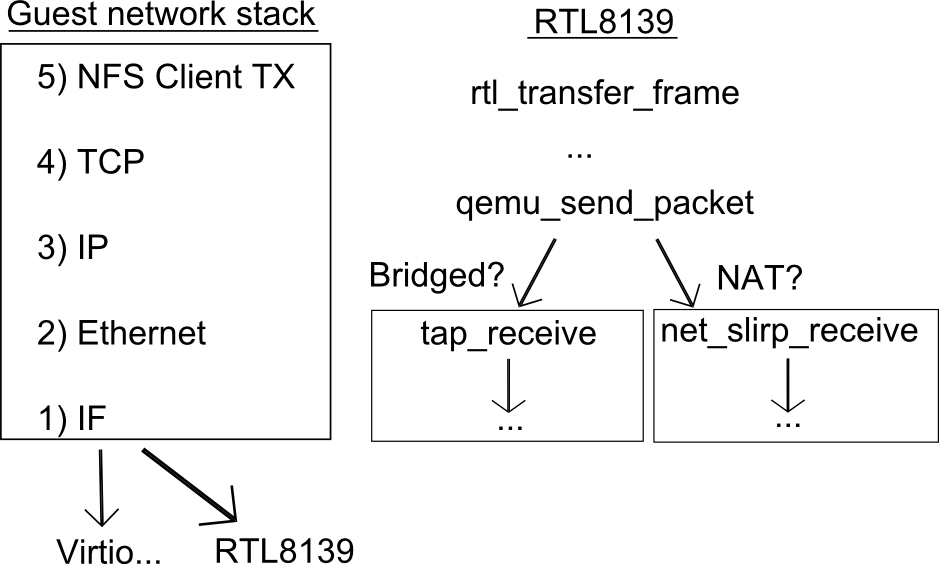
\includegraphics[scale=0.6]{codepath1}
	\caption{Virtualized client TX code path under bridged and user-mode (NAT) networking using the RTL8139 fully emulated driver. Both start at the top of the guest network stack, but diverge after \texttt{qemu\_deliver\_packet}.}
	\label{fig:codepath1}
\end{figure*}

\begin{figure*}[!ht]
	\centering
		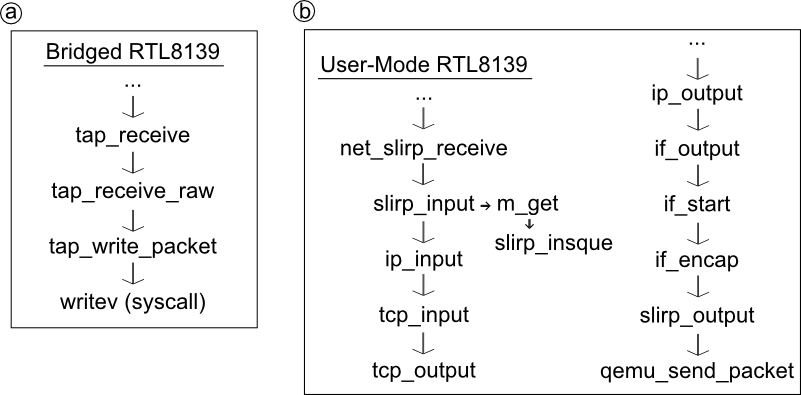
\includegraphics[scale=0.6]{codepath2_alt}
	\caption{Important functions in the divergent branches of bridged and user-mode networking.}
	\label{fig:codepath2}
\end{figure*}

Figure \ref{fig:codepath2}b shows a flowchart of functions that a packet passes through when a guest VM sends a packet to the Internet while using usermode networking.
The control flow starts with the RealTek driver passing the packet to the \texttt{slirp\_input} function.
\texttt{Slirp\_input} calls two functions before the control flow continues, \texttt{m\_get} which in turn calls \texttt{slirp\_insque}.
In \texttt{m\_get}, memory is allocated and then passed on to \texttt{slirp\_insque} to be added a doubly linked list which acts as a packet buffer.
The chunk of memory is then returned to \texttt{slirp\_output} where the packet is then copied into it. % TODO: reword
It is this allocating, managing, and copying of memory done for every packet in these three functions that causes the majority of the slowdown in usermode networking.

Once the packet has been copied into the buffer space, it is passed ``up the stack'' to \texttt{ip\_input}. 
The function uses the packet's IP headers to sanity check different aspects such as the checksum and length.
Then, IP options are processed and if the packet is fragmented, it attempts to reassemble it.
If the packet is malformed then it is dropped and the memory used to store it is freed.

If the packet passes the tests in \texttt{ip\_input} it is passed along to \texttt{tcp\_input}.
\texttt{Tcp\_input} is a direct implementation of the TCP specification from September, 1981.
It does all the standard operations associated with TCP such as calculating the receive window and updating the TCP control block that QEMU maintains.
It then strips both the IP and TCP headers from the packet, leaving just the TCP payload, which is passed to \texttt{tcp\_output}.
It is at this point that the packet starts to move back ``down the stack'' to be put out onto the wire.
\texttt{Tcp\_output} handles TCP timers which determine when a packet should actually be sent.
Once a packet is cleared to be sent, the TTL and TOS fields are filled in and the packet is passed along.

With the transport layer complete the packet moves to the \texttt{ip\_output} where the packet's IP header fields filled in with the host's information.
At this point the packet is fully formed and ready to put on the wire.
It is handed off to \texttt{if\_output} which manages two different packet queues, \texttt{fastq} and \texttt{batchq}.
If a packet has the \texttt{IPTOS\_LOWDELAY} flag set, then it is placed on the \texttt{fastq}, which is intended for packets from an interactive application.
Otherwise, the packet is placed on the \texttt{batchq}.
``Each output queue is a doubly linked list of doubly linked lists of mbufs, each list belonging to a separate socket.''
If a socket is found that does not have a linked list yet, then another is created and the packet is added to this new linked list.
To create the linked list, \texttt{if\_output} calls \texttt{m\_get} which in turn calls \texttt{slirp\_insque}.

The packet then moves on to \texttt{if\_start} which services both the \texttt{fastq} and the \texttt{batchq}.
As the names would indicate, the \texttt{fastq} is serviced first.
This function passes the packets from the queues on and then cleans up memory upon return through the \texttt{m\_free} and \texttt{slirp\_remque} functions.

When a packet is serviced it is passed to \texttt{if\_encap}.
Here the packet is prepared for going out on the wire by copying the packet header information into the appropriate header structs.
Finally the packet is passed along to \texttt{slirp\_output}. 
Essentially \texttt{slirp\_output} just puts the packet on whatever queue is passed into it along with additional slirp state information.
This is done by simply calling \texttt{qemu\_send\_packet}.
At this point qemu takes over and the rest of the control path is no longer dictated by the fact that usermode networking is in use.

\subsection{RealTek 8139 Bridged: Guest Transmit}
Perhaps not surprisingly, the main code path of the RealTek 8139 under bridged networking is substantially more straightforward.  

The packet first comes out the end of the shared code (see Appendix) and is sent by \texttt{qemu\_deliver\_packet} to \texttt{tap\_receive}. \texttt{Tap\_receive} then performs some header checks and sends the packet to \texttt{tap\_receive\_raw}, which breaks the packet into IO vectors and sends it to \texttt{tap\_write\_packet}. That function is simply a wrapper around the \texttt{writev} system call, which writes the packet out to the TAP device. 

As we can see, the bridged networking code is much simpler and performs only minimal memory accesses, making it a great deal faster than user-mode networking. 

\subsection{Code Path Timing}
\label{codePathTiming}
We timed the diverging sections of user-mode and bridged networking transmission paths. We began timing both paths at the function \texttt{rtl8139\_transfer\_frame}, ending the user-mode timing at \texttt{slirp\_output} and the bridged timing at function \texttt{tap\_write\_packet}. The user-mode path took an average of 1.1 milliseconds, while the bridged path took an average of 44 microseconds, demonstrating a factor of 25 slowdown for user-mode networking relative to bridged.

\begin{figure}[!htbp]
	\centering
		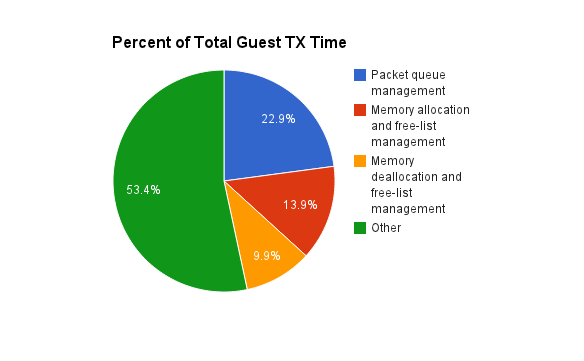
\includegraphics[scale=0.5]{usermodeTXtime}
	\caption{Almost half of the time spent in user-mode networking is spent in memory management.}
	\label{fig:usermodeTXtime}
\end{figure}

We found that almost 50\% of the overhead in user-mode networking is due to the memory management that takes place in \texttt{slirp\_input}, \texttt{if\_output}, and \texttt{if\_input}. The use of NAT in SLiRP means that a packet has to travel down the guest network stack, and then back up and down the network stack in SLiRP as it gets deencapsulated and reencapsulated with the host's network information, before finally getting sent to the host network stack. The memory management involved in this process---managing doubly linked lists of doubly linked lists of mbufs containing the packet information---necessarily incurs substantial overhead. 
